\documentclass[a4paper,12pt]{article} % Tipo de documento y tamaño de letra.
\usepackage[utf8]{inputenc} % Para que reconozca caracteres especiales como tildes.
\usepackage[spanish]{babel} % Para definir el idioma y el formato de fechas en español.
\usepackage{amsmath, amssymb} % Paquetes para símbolos y ecuaciones avanzadas (Para hacer una ecuación con un recuadro).
\usepackage{ragged2e} % Para justificar textos.
\usepackage{multicol} % Para crear columnas.
\usepackage{slashed} % Para generar números o variables canceladas (Una línea diagonal sobre el número o variable).
\usepackage{graphicx} % Paquete para poner graficas.
\usepackage{float} % Para poder dejar la imagen en un punto fijo del documento.
\usepackage{longtable} % Para tablas largas.
\usepackage{cancel} % Para hacer cancelaciones en medio de operaciones.
\usepackage{xcolor} % Para el color y esas cosas.
\usepackage{apacite} % Paquete para citas APA.
\usepackage{fancyhdr} % Para personalizar encabezados y pies de página.
\usepackage{geometry} % Para ajustar márgenes.
\usepackage{setspace} % Para ajustar el interlineado.
\usepackage{natbib} % Para manejar las citas y que no queden pegadas y feas :P.
\usepackage{hyperref} % Para que los enlaces funcionen con su URL.
\usepackage[version=4]{mhchem}  % Versión recomendada para mayor funcionalidad.
\usepackage{chemfig} %También para hacer estructuras químicas.
\usepackage{array} % Para mejor control de las columnas.
\usepackage{siunitx} % Para unidades físicas.


\pagestyle{fancy}
\fancyhf{} % Limpia encabezados y pies de página predeterminados
\fancyhead[L]{\textbf{SIMULACIONES.}} % Encabezado izquierdo
\fancyhead[R]{\textbf{FÍSICA ll}} % Encabezado derecho
\fancyfoot[C]{\thepage} % Número de página en el centro del pie

\geometry{headheight=12.96115pt, top=1in, bottom=1in, left=1in, right=1in}
\begin{document}

\begin{figure}[H] 
    \centering
    
\includegraphics[width=0.5\textwidth]{Unir.jpg} 
\end{figure}

\vspace{\baselineskip}

% Ajustamos manualmente todo ;)
\begin{center}
    \textbf{\Large } \\[0.3cm]
    \vspace{\baselineskip}
    \textbf{Liz Ángel Núñez Torres} \\[0.4cm]
    \textbf{Grado en Física} \\[0.4cm]
    \textbf{Universidad Internacional de La Rioja} \\[0.4cm]
    \textbf{19 de Marzo de 2025}
\end{center}



\newpage

\tableofcontents

\newpage



\section{Ejercicio 1: Simulación de un oscilador armónico.}

\begin{justify}
    En clase, hemos visto que un oscilador armónico sigue la ecuación diferencial
\end{justify}

\[
\frac{d^{2}x}{dt^{2}} = -\omega^{2}x.
\]

\begin{justify}
Las soluciones armónicas a esta ecuación son del tipo \(x(t) = A\cos(\omega t - kx)\). Ahora, queremos resolver numéricamente esta ecuación para un valor particular de \(\omega\) y vamos a comprobar qué diferencia hay entre la solución numérica y la solución analítica. Para ello, vamos a escribir la ecuación diferencial como
\end{justify}

\[
\frac{dx}{dt} = v, \quad \frac{dv}{dt} = -\omega^{2}x.
\]

\begin{justify}
Esto nos permite resolverla numéricamente usando diferentes métodos de integración. Una vez tenemos calculadas las soluciones numérica y analítica, podemos comparar sus valores para ver si son iguales. Para ello, calculamos el error absoluto, esto es, \(x_{\textrm{analítico}} - x_{\textrm{numérico}}\).
\end{justify}

\begin{enumerate}
    \item Averigua qué método numérico está utilizando \texttt{solve\_ivp} por defecto. ¿Cambia el resultado si probamos otros métodos, como Runge-Kutta de orden 3 (\texttt{solver='RK23'}) o Dormand-Prince (\texttt{solver='DOP853'})?
    
    \item ¿Cómo afecta el número de puntos en \texttt{t\_eval} al error numérico? ¿Qué pasa si usamos 100 o 20 puntos en lugar de 1000? ¿Y 10000 en vez de 1000?
    
    \item ¿Qué representa físicamente la curva de error? ¿Hay algún patrón? Discute qué sucede si simulamos tiempos muy grandes.
    
    \item Cambia el parámetro de \(\omega\) para tal que la simulación corresponda a un oscilador armónico con \(k = \textrm{el número}\) correspondiente a la primera letra de tu nombre (\(A=1, B=2\), ...) y \(m = \textrm{el número}\) correspondiente a la primera letra de tu nombre. Debes adaptar el intervalo de tiempo de la simulación para que tu resultado sea lo más claro posible. Adjunta la gráfica de la solución a tu respuesta.
    
    \item Haz que \(\omega\) sea una función del tiempo, por ejemplo, \(\omega(t) = 1 + \Omega\sin(t), \Omega \in (0,50)\). Comprueba que cuando \(\Omega \approx 0\) se recupera un oscilador armónico normal, mientras que para valores altos de \(\Omega\) el resultado es más exótico.
    
    \item Obtén la constante de fuerza del enlace de una molécula de \(O_{2}\). Esto puede hacerse sabiendo que la frecuencia fundamental de vibración del oxígeno molecular es aproximadamente \(f = 4.7 \times 10^{13}\) Hz, y que la masa de cada uno de los oxígenos es de \(m = 2.66 \times 10^{-26}\) kg. Vamos a suponer que la molécula se comporta como un oscilador armónico simple, con ambos átomos conectados por un resorte ideal. En tal caso, la frecuencia angular es \(\omega = \sqrt{\frac{k}{\mu}}\), donde \(\mu\) es la masa reducida. Una vez tengas \(k\), simula el movimiento de la molécula, ajustando \texttt{t\_span} y \texttt{t\_eval}.
\end{enumerate}

\subsection{Método númerico.}

\vspace{\baselineskip}

\begin{justify}
    El método por defecto de \verb|solve_ivp| es \verb|RK45| (Runge-Kutta de orden 4/5), que es una variante del método de Dormand-Prince. Si no especificas el parámetro \verb|solver|, se usará \verb|RK45|. 
\end{justify}

\begin{justify}
    \textbf{¿Cambia el resultado si usamos otros métodos?}
\end{justify}

\vspace{\baselineskip}

\begin{itemize}
    \item \textbf{Método:} \verb|RK45| (Por defecto).
\end{itemize}
\begin{figure}[H]
    \centering
    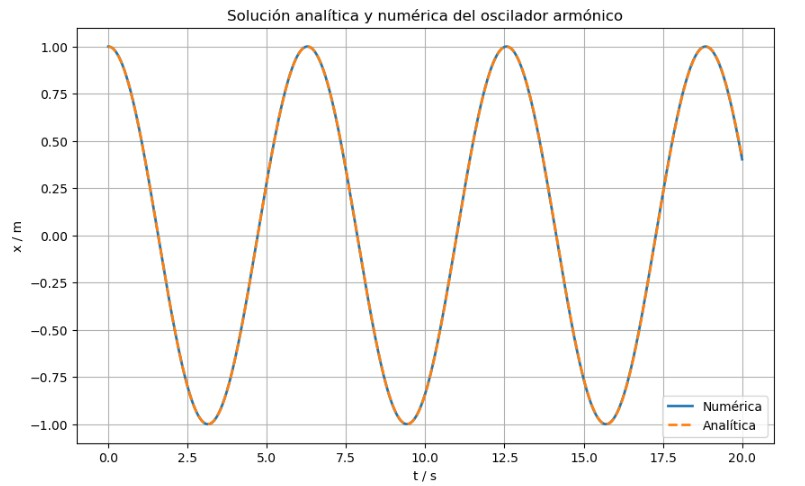
\includegraphics[width=0.5 \textwidth]{lab1.jpg}
    \caption{Gráfica del método por defecto.}
\end{figure}

\vspace{\baselineskip}

\begin{itemize}
    \item \textbf{Método:} \verb|RK23| Runge-Kutta de orden 3.
\end{itemize}
\begin{figure}[H]
    \centering
    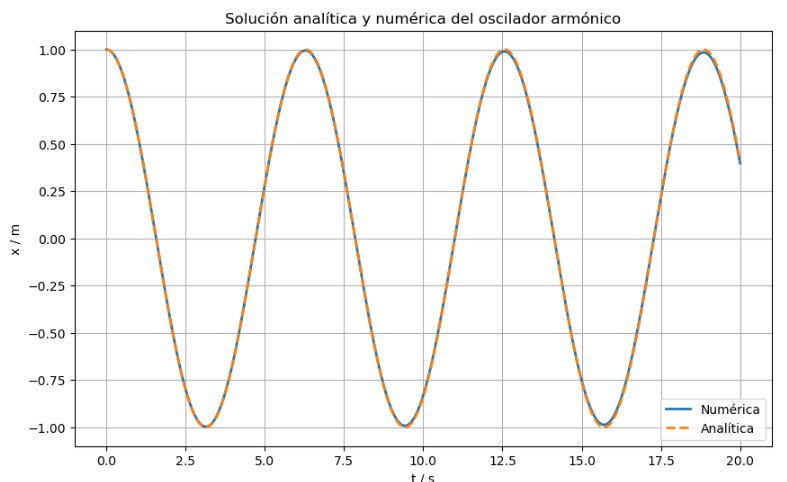
\includegraphics[width=0.5 \textwidth]{lab2.jpg}
    \caption{Gráfica del método RK23 de orden 3.}
\end{figure}

\vspace{\baselineskip}

\begin{itemize}
    \item \textbf{Método:} \verb|DOP853| Runge-Kutta de orden 8 .
\end{itemize}
\begin{figure}[H]
    \centering
    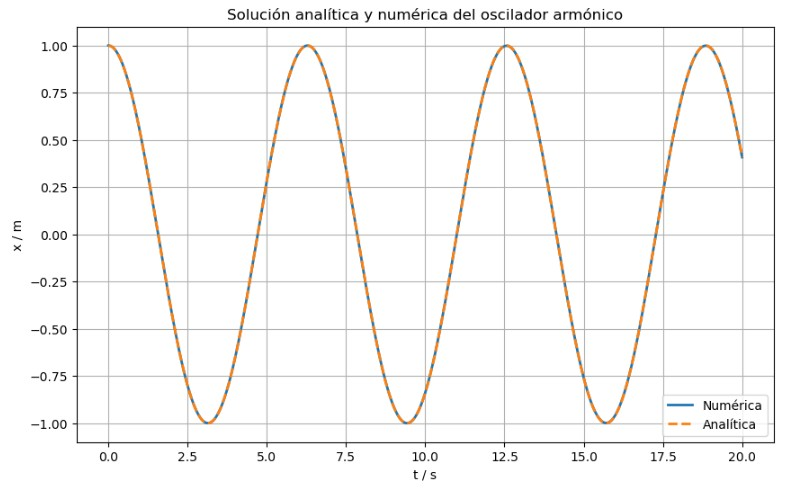
\includegraphics[width=0.5 \textwidth]{lab3.jpg}
    \caption{Gráfica del método DOP853 de orden 8.}
\end{figure}

\begin{justify}
    Como podemos observar, no se aprecia un cambio considerable más allá del suavizado en la gráfica sinusoidal, esto es debido que la solución 
    analítica (\textbf{donde si existe un cambio númerico}) es suave, además el error es muy pequeño del orden de \(10^{-6}\) o menos, lo que ocasione que no sea facilmente perceptible el cambio de método.
    Cabe resaltar, que en la imagen \textit{``Error absoluto entre la solución numérica y la solución analítica''} \textbf{ no se presenta ningún cambio más allá de la calidad de las lineas} al igual que en las graficas anteriormente expuestas.
\end{justify}

\vspace{\baselineskip}

\subsection{¿Cómo afecta el número de puntos en t\_eval al error numérico?}

\vspace{\baselineskip}

\begin{justify}
    Vamos a mostrar como afecta \verb|t_eval| al error numérico con \(20\) puntos y con \(10000\) puntos, debido que este enorme intervalo de puntos nos
    genera una apreciación más solida para argumentar esta variación.
\end{justify}

\begin{itemize}
    \item Error númerico cuando \verb|t_eval| \(\Rightarrow\) \verb|nt| \(= 20.\)
\end{itemize}
\begin{figure}[H]
    \centering
    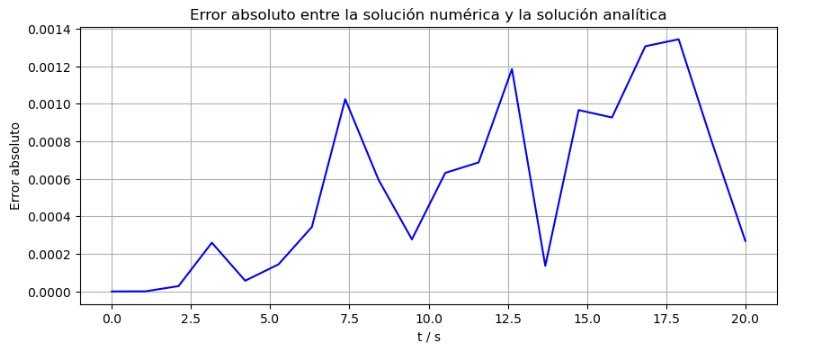
\includegraphics[width=0.7 \textwidth]{err1.jpg}
    \caption{Gráfica ``Error absoluto entre la solución numérica y la solución analítico'' con 20 puntos.}
\end{figure}

\vspace{\baselineskip}

\begin{itemize}
    \item Error númerico cuando \verb|t_eval| \(\Rightarrow\) \verb|nt| \(= 20.\)
\end{itemize}
\begin{figure}[H]
    \centering
    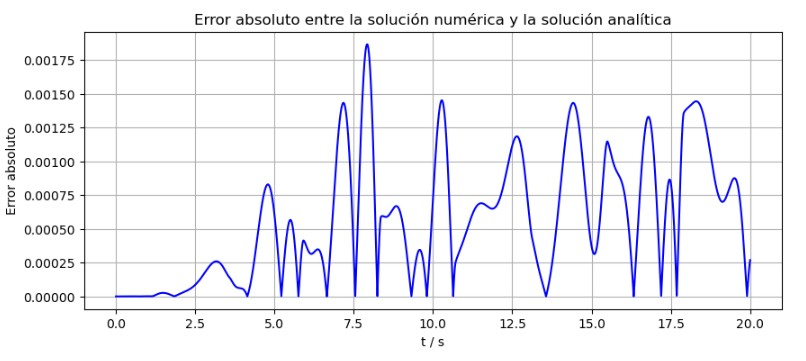
\includegraphics[width=0.7 \textwidth]{err2.jpg}
    \caption{Gráfica ``Error absoluto entre la solución numérica y la solución analítico'' con 1000 puntos.}
\end{figure}

\vspace{\baselineskip}

\begin{justify}
    Como podemos observar en las imagenes, nuestras gráficas cambian de \textbf{escalonada} a más \textbf{suave} especialmente en los picos.
    Esto es debido que al \textbf{disminuir los puntos, aumenta el error númerico} y  al \textbf{aumentar los puntos, disminuye el error númerico}; podemos argüir que existe una relación \textbf{inversamente proporcional a los puntos.} 
\end{justify}

\vspace{\baselineskip}

\subsection{¿Qué representa físicamente la curva de error? ¿Hay algún patrón?}

\vspace{\baselineskip}

\begin{justify}
    La curva de error representa la discrepancia entre el método númerico y la verdadera solución, estos errores ocurren por:
\end{justify}

\begin{itemize}
    \item \textbf{Método:} Como hemos visto antes, existen métodos de menor orden, como \verb|RK23| que es orden 3, lo cual afecta a su precisión, por esto, para una solución más exacta, recomendamos usar métodos del orden 8, como lo es \verb|DOP853|.
    \item \textbf{Discretización temporal} Al usar pasos finitos en lugar de infinitamente pequeños (como pudimos constatar en nuestro anterior apartado), se pierde información entre puntos.
\end{itemize}

\vspace{\baselineskip}

\begin{justify}
    Podemos ver en linea de código (\texttt{error = np.abs(\(sol.y[0]\) - \(x_{analytic}\))}) que mide la diferencia entre la \textbf{solución númerica} (\texttt{sol}) y la \textbf{solución analítica} (\texttt{\(x_{analytic}\)}).
\end{justify}

\vspace{\baselineskip}

\begin{justify}
    Si modificamos el tiempo obtenemos que:
\end{justify}

\vspace{\baselineskip}

\begin{itemize}
    \item \textbf{Tiempo} \texttt{t\_span} = 0, 100. 
    
    \begin{figure}[H]
        \centering
        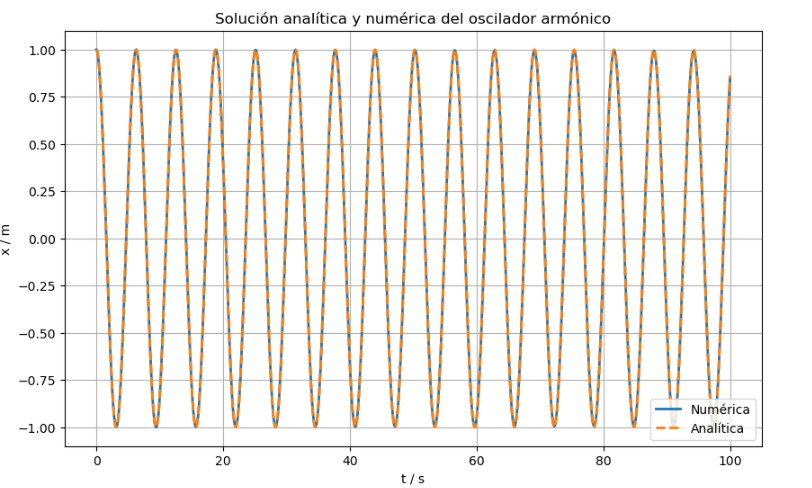
\includegraphics[width=0.7 \textwidth]{t1.jpg}
        \caption{Tiempo 100 con método \texttt{DOP853} y \texttt{nt} = 1000.}
    \end{figure}
\end{itemize}

\vspace{\baselineskip}

\begin{itemize}
    \item \textbf{Tiempo} \texttt{t\_span} = 0, 1000. 
    
    \begin{figure}[H]
        \centering
        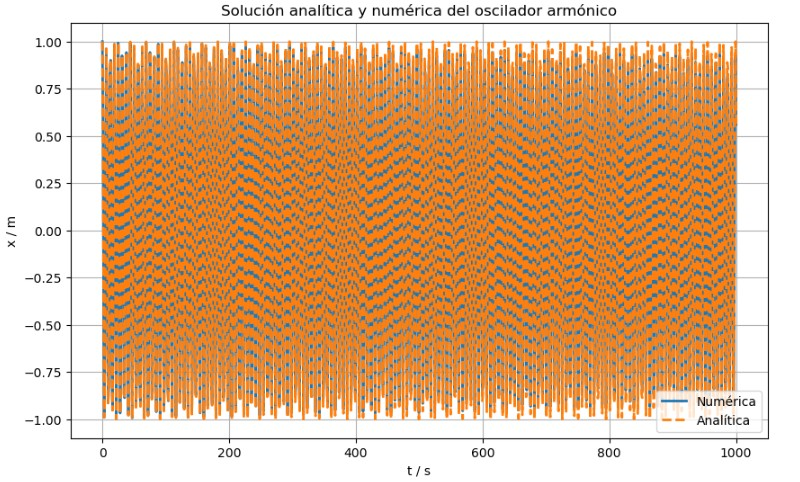
\includegraphics[width=0.7 \textwidth]{t2.jpg}
        \caption{Tiempo 1000 con método \texttt{DOP853} y \texttt{nt} = 1000.}
    \end{figure}
\end{itemize}

\vspace{\baselineskip}

\begin{justify}
    El \textbf{patrón} y conclusión \textbf{respecto al tiempo} es que el error absoluto entre la solución númerica y analítica crece con el tiempo como podemos observar en la \texttt{Figura 7} con t\_span = 1000. 
\end{justify}

\vspace{\baselineskip}

\subsection{Parámetro \(\omega\) .}

\vspace{\baselineskip}

\begin{justify}
    Modificamos \( \omega\) donde \textbf{L} = 12.
\end{justify}


\begin{figure}[H]
    \centering
    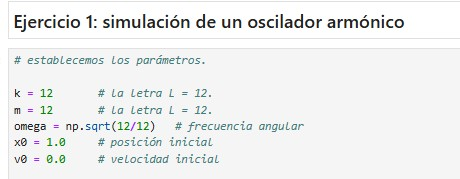
\includegraphics[width=0.7 \textwidth]{L1.jpg}
    \caption{Sustitución de \(\omega\) por \(\sqrt{\frac{k}{m}} \)}
\end{figure}

\vspace{\baselineskip}

\begin{justify}
    Modificamos el tiempo por \textbf{dos ciclos completos.}

\end{justify}


\begin{figure}[H]
    \centering
    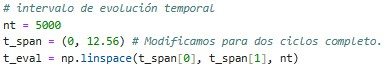
\includegraphics[width=0.7 \textwidth]{L2.jpg}
    \caption{Sustitución del tiempo por 2 ciclos completos. }
\end{figure}

\vspace{\baselineskip}

\begin{justify}
    Grafica con \(\omega = \sqrt{\frac{12}{12}}\).
\end{justify}


\begin{figure}[H]
    \centering
    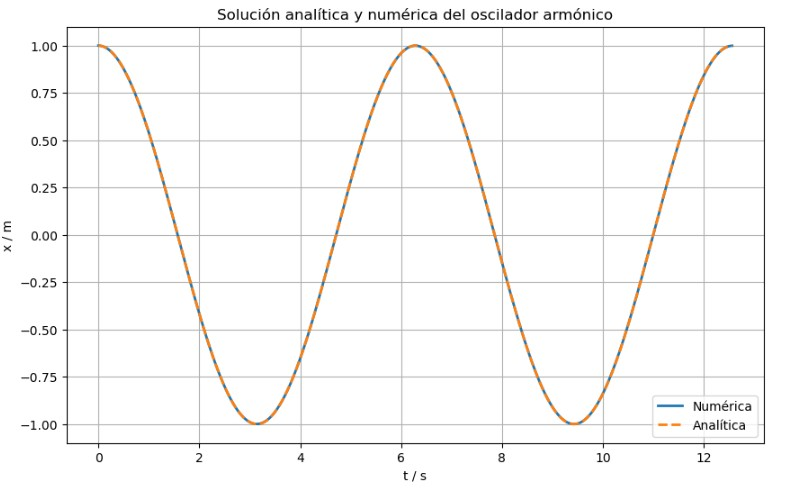
\includegraphics[width=0.7 \textwidth]{sol.jpg}
    \caption{ \( \omega = 1 \) con 2 \(\pi\) ciclos. }
\end{figure}

\begin{justify}
    Aunque hemos modificado \( \omega \) esta sigue siendo la misma númerica mente debido que nuestra raíz es igual a 1, al modificar el tiempo podemos encontrar la correlación entre la sólución númerica y analítica 
    sin embargo no presenta un cambio perceptible en la grafica.
\end{justify}

\vspace{\baselineskip}

\subsection{Omega (\( \omega\)) en función del tiempo. }

\vspace{\baselineskip}

\begin{justify}
    Para este punto definimos una variable \texttt{\(\Omega\) = 0} más la definición de \( \omega\) en función del tiempo.
\end{justify}

\vspace{\baselineskip}

\begin{figure}[H]
    \centering
    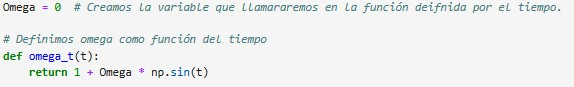
\includegraphics[width=0.9 \textwidth]{om1.jpg}
    \caption{ Omega \( \omega\) en función del tiempo. }
\end{figure}

\vspace{\baselineskip}

\begin{justify}
    Como podemos obsevar en el código, definimos \( \Omega = 0 \) lo que genera que nuestra gráfica de la solución analítica y numérica del oscilador armónico 
    \textbf{no cambie}.
\end{justify}

\begin{figure}[H]
    \centering
    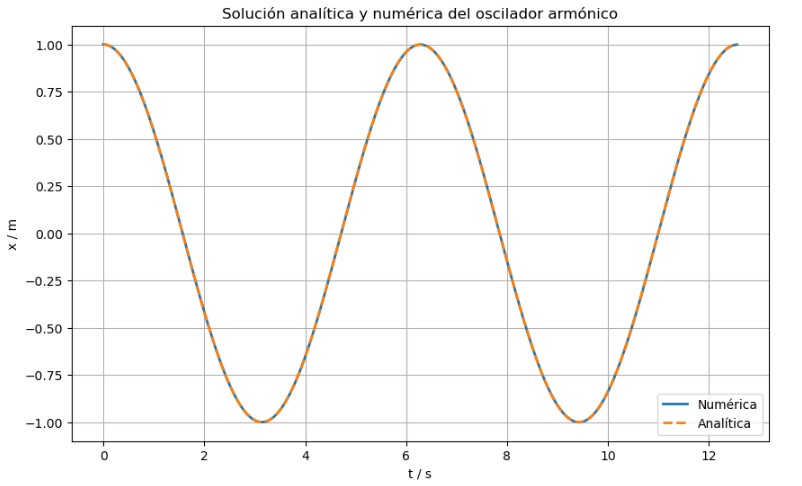
\includegraphics[width=0.8 \textwidth]{om2.jpg}
    \caption{ No se obtiene ningún cambio al definir \( \Omega = 0 \). }
\end{figure}

\vspace{\baselineskip}

\begin{justify}
    Al definir \( \Omega > 0 \) genera que nuestra gráfica de la solución analítica y numérica del oscilador armónico presente un desface.
    Esto es porque cambiamos de un \textbf{oscilador amónico clásico} donde la frecuencia es constante a un \textbf{oscilador paramétrico} con la frecuencia dependiente del tiempo.
\end{justify}


\begin{figure}[H]
    \centering
    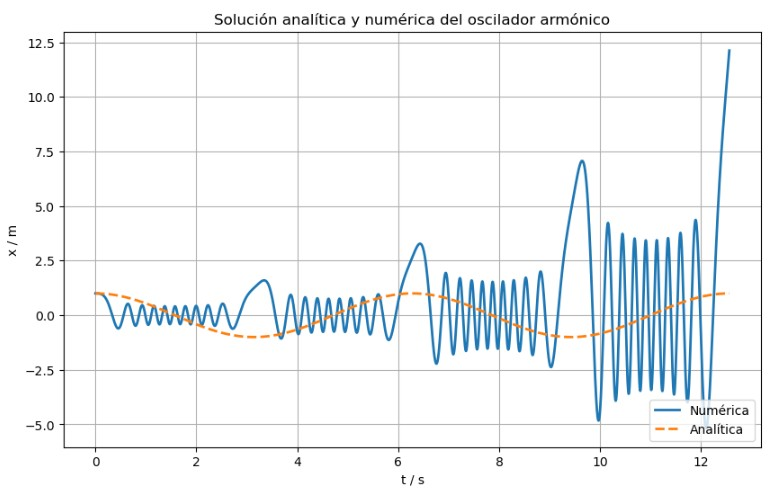
\includegraphics[width=0.8 \textwidth]{om3.jpg}
    \caption{ Cuando \(\Omega  = 30\). }
\end{figure}

\subsection{Fuerza de enlace de una molécula de óxigeno \ce{O2}.}


\begin{justify}
    Adjuntamos los datos a nuestro código, despejamos \( \omega \) y obtenemos el valor de \(k\).
\end{justify}

\begin{figure}[H]
    \centering
    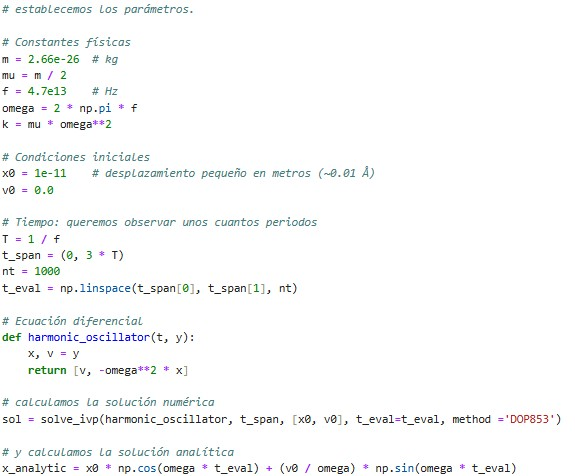
\includegraphics[width=0.7 \textwidth]{O2.jpg}
    \caption{ Datos de la molécua \ce{O2} y depseje de \(k\). }
\end{figure}

\begin{justify}
    Y la gráfica obtenida de la fuerza de enlace es:
\end{justify}

\begin{figure}[H]
    \centering
    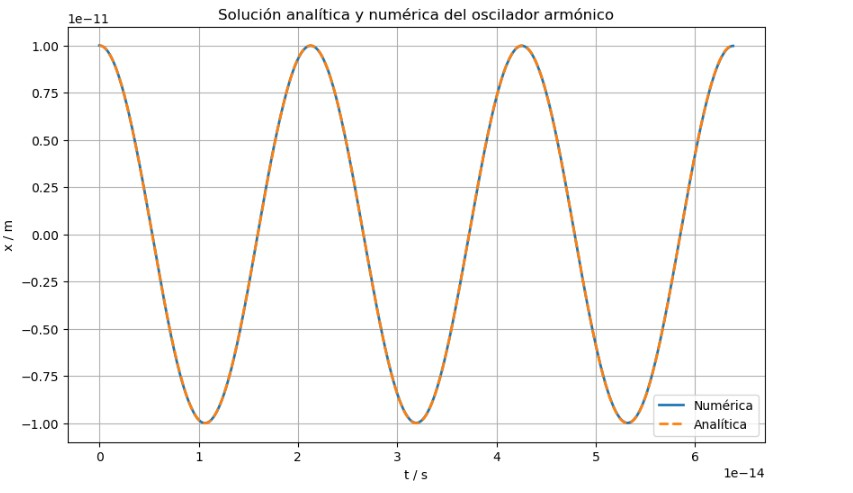
\includegraphics[width=0.7 \textwidth]{O3.jpg}
    \caption{ Datos de la molécua \ce{O2} y depseje de \(k\). }
\end{figure}

\vspace{\baselineskip}

\section{ Ejercicio 2: Energía del oscilador armónico.}

\begin{justify}
Este ejercicio trata del mismo problema que el anterior, pero vamos a enfocarnos en su energía. Además, aprovechamos para ver cómo podemos hacer una animación en Python, la cual nos ayuda a ver con mayor claridad la evolución temporal del sistema.
\end{justify}

\begin{enumerate}
    \item Cambia los parámetros de la simulación a unos valores elegidos por ti y adjunta la nueva figura resultante. ¿Cuál es el valor máximo de la energía cinética? ¿Y de la potencial? ¿Cuándo se alcanzan estos valores? ¿Y de la energía total? ¿Es este el comportamiento que esperabas? Relaciona los máximos de energía cinética y potencial con la velocidad y aceleración.
    
    \item Introducid un amortiguamiento proporcional a la velocidad (resistencia viscosa), lo cual puede ser modelizado tomando \(a = -\omega^{2}x(t) - \gamma v^{2}\), con \(\gamma\) una constante arbitraria. Adjunta la figura resultante. Comenta cómo evoluciona la energía en este caso.
\end{enumerate}

\newpage

\subsection{Parámetros  de simulación.}

\vspace{\baselineskip}

\begin{justify}
    Modificamos los parámetros.
\end{justify}

\begin{figure}[H]
    \centering
    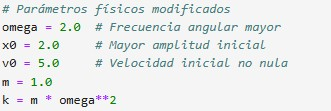
\includegraphics[width=0.6 \textwidth]{par1.jpg}
    \caption{Parámetros modificados.}
\end{figure}

\vspace{\baselineskip}

\begin{justify}
    \textbf{La imagen obtenida es:}
\end{justify}

\vspace{\baselineskip}

\begin{figure}[H]
    \centering
    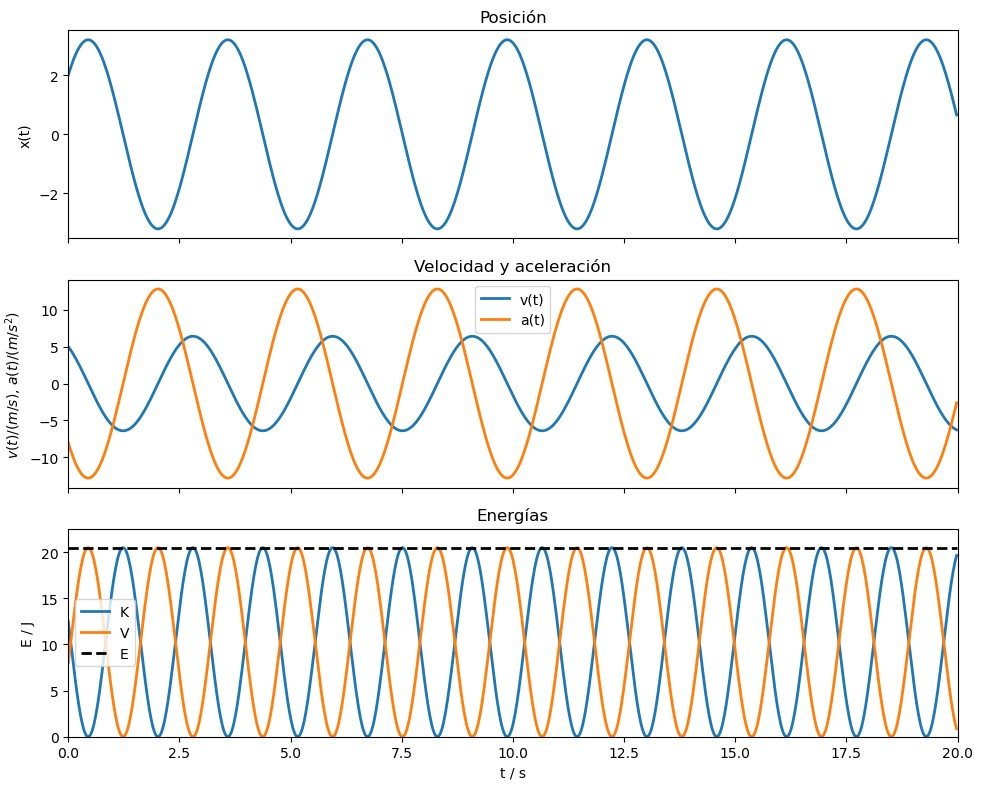
\includegraphics[width=0.9 \textwidth]{par2.jpg}
    \caption{Gráfica de la nueva simulación.}
\end{figure}

\newpage 

\begin{justify}
    \textbf{¿Cuál es el valor máximo de la energía cinética y cuando se alcanza?}
\end{justify}

\begin{itemize}
    \item \texttt{K\_max} \(\rightarrow 16.5 \; J\). Se alcanza cuando la posición en \(x = 0\), que es el punto de equilibrio. Coincide con los momentos de máxima velocidad
    que dependiendo de su dirección será \textbf{positiva o negativa}. \(( v = \pm \; 5.66 \; m/s)\)
\end{itemize}

\begin{justify}
    \textbf{¿Cuál es el valor máximo de la energía potencial y cuando se alcanza?}
\end{justify}

\begin{itemize}
    \item \texttt{U\_max} \(\rightarrow 8.0 \; J\) Se alcanza en los puntos de máxima elongación. Coincide con los momentos donde la velocidad es cero. \(( x = \pm \; 2.83 \; m)\)
\end{itemize}

\begin{justify}
    \textbf{Energía total (E) ¿Esperabamos este resultado?}
\end{justify}

\begin{itemize}
    \item Constanten en \( 16.5 \; J \). Es lo que esperabamos, dado que es un oscilador amónico \textbf{sin amortiguamiento.}
\end{itemize}

\vspace{\baselineskip}

\subsection{Amortiguamiento porporcional a la velocidad.}

\vspace{\baselineskip}

\begin{justify}
    Creamos una variable \texttt{(gamma  = 0.5)} y modificamos, \texttt{(a = -omega**2 * x)} en \texttt{(a = -omega**2 * x - gamma * v**2)}.
\end{justify}

\vspace{\baselineskip}

\begin{figure}[H]
    \centering
    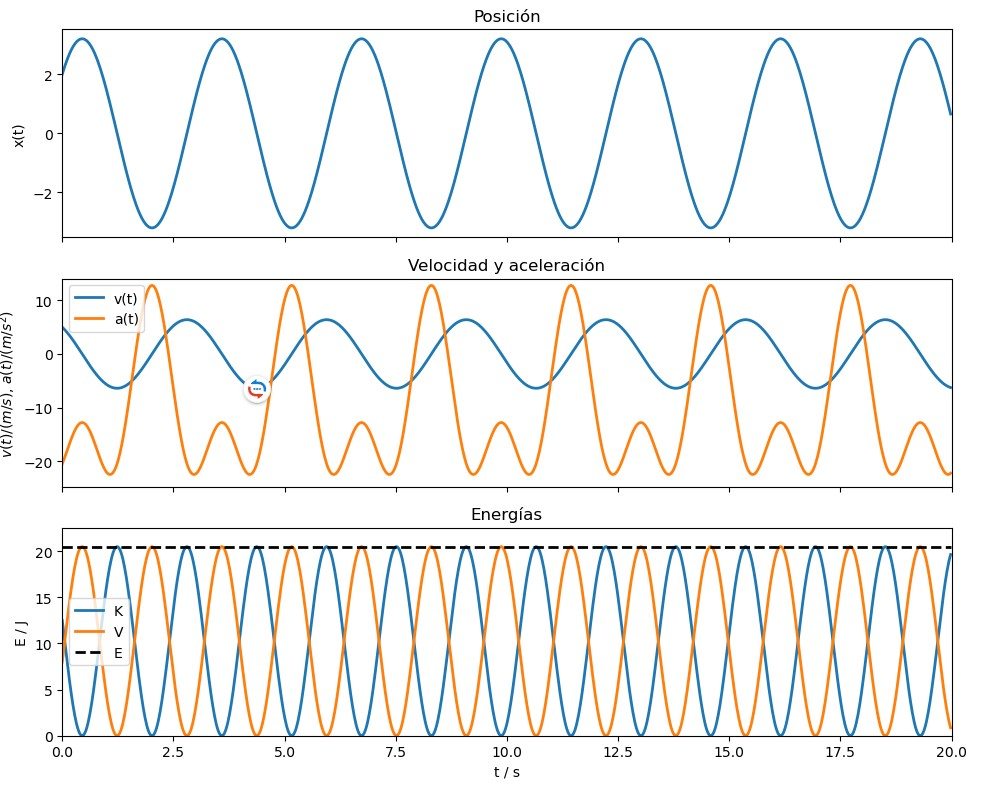
\includegraphics[width=0.8 \textwidth]{am1.jpg}
    \caption{Gráfica con \(\gamma\) constante y \(a = - \omega^2 \cdot x - \gamma \cdot v^2\).}
\end{figure}

\vspace{\baselineskip}

\section{ Ejercicio 3: Pulso en una cuerda.}

\begin{justify}
Un hombre está tendiendo la ropa en unas cuerdas y se da cuenta de que, al subir y bajar uno de los extremos de la cuerda se genera un pulso que se aleja de él. Este, al llegar al otro extremo de la pared, es reflejado de vuelta hacia el hombre. Para entender mejor el suceso, el hombre decide hacer una simulación en el ordenador.
\end{justify}

\begin{enumerate}
    \item Ejecuta la simulación. Una vez la ejecutes, cambia los parámetros del pulso inicial (\texttt{sigma}, \texttt{x0}...). Adjunta la animación resultante.
    
    \item Modifica el pulso inicial (función \texttt{initial\_pulse} en el código) para que en vez de un pulso a la izquierda, también haya otro pulso a la derecha. Debes simular el caso en el que este segundo pulso tiene amplitud positiva y el caso con amplitud negativa. Explica cómo interfieren las ondas en cada caso.
    
    \item Modifica el impulso inicial para tal que sea una onda cuadrada (por ejemplo, \texttt{np.where(x > 0.4) \& (x < 0.6), 1.0, 0.0)}. Adjunta una figura de tus resultados. Comenta el resultado.
\end{enumerate}

\vspace{\baselineskip}

\subsection{Parámetros del pulso inicial.}

\vspace{\baselineskip}

\begin{justify}
    Ajustamos el pulso inicial.  \texttt{x0=0.5} y \texttt{sigma=0.09} (Se adjuntará esta y las demás animaciones en un archivo aparte.)
\end{justify}

\begin{figure}[H]
    \centering
    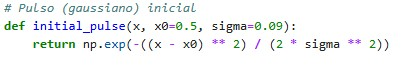
\includegraphics[width=0.7 \textwidth]{pul1.jpg}
    \caption{Modificación del pulso gaussiano.}
\end{figure}

\newpage

\begin{justify}
    Siendo nuestra gráfica:
\end{justify}

\begin{figure}[H]
    \centering
    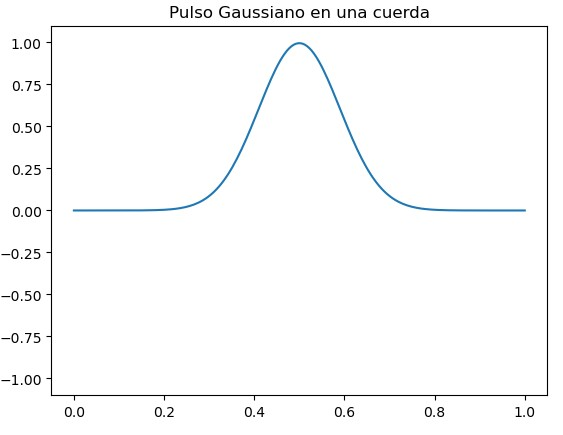
\includegraphics[width=0.7 \textwidth]{pul3.jpg}
    \caption{Pulso gaussiano.}
\end{figure}

\vspace{\baselineskip}

\subsection{Modificación del pulso inicial.}

\vspace{\baselineskip}

\begin{justify}
    Modificamos la función \texttt{initial\_pulse} e incluimos dos pulsos.
\end{justify}

\begin{figure}[H]
    \centering
    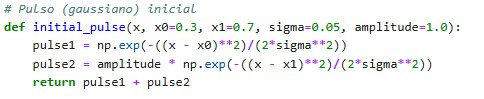
\includegraphics[width=0.7 \textwidth]{pul2.jpg}
    \caption{Modificación del pulso gaussiano.}
\end{figure}

\newpage

\begin{justify}
    \textbf{Figura con la amplitud positiva.} 
\end{justify}


\begin{figure}[H]
    \centering
    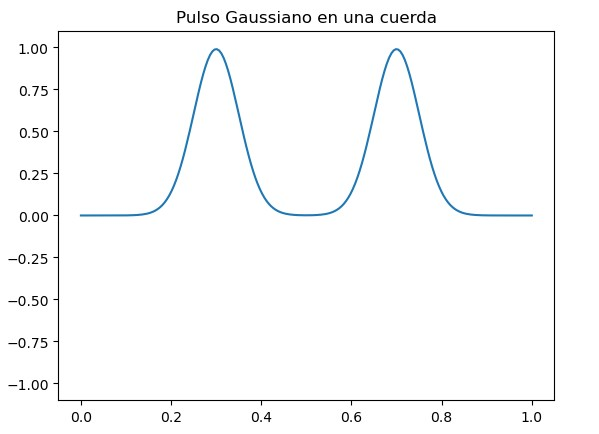
\includegraphics[width=0.7 \textwidth]{pul4.jpg}
    \caption{Modificación del pulso gaussiano con amplitud positiva.}
\end{figure}

\vspace{\baselineskip}

\begin{justify}
    Cuando el segundo pulso tiene amplitud positiva, las ondas se interfieren \textbf{constructivamente}
    cuando se encuentran en el centro. La amplitud resultante es la suma de ambas ondas.
\end{justify}

\vspace{\baselineskip}

\begin{justify}
    \textbf{Figura con la amplitud negativa.}
\end{justify}


\begin{figure}[H]
    \centering
    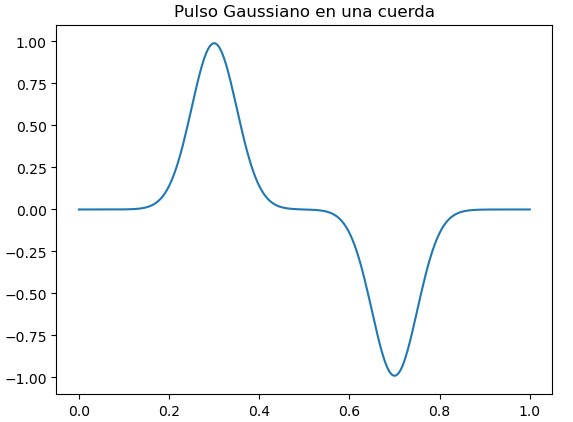
\includegraphics[width=0.7 \textwidth]{pul5.jpg}
    \caption{Modificación del pulso gaussiano con amplitud negativa.}
\end{figure}

\vspace{\baselineskip}

\begin{justify}
    Cuando el segundo pulso tiene amplitud negativa, las ondas interfieren \textbf{destructivamente} cuando se encuentran,
    cancelñandose parcial o totalmente dependiendiendo de la fase exacta.
\end{justify}

\vspace{\baselineskip}

\subsection{Pulso inicial - onda cuadrada.}

\vspace{\baselineskip}

\begin{justify}
    Modificamos el pulso inicial:
\end{justify}

\begin{figure}[H]
    \centering
    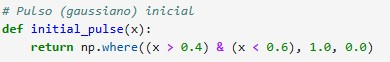
\includegraphics[width=0.7 \textwidth]{pul6.jpg}
    \caption{Modificación del pulso gaussiano en onda cuadrada.}
\end{figure}

\vspace{\baselineskip}

\begin{justify}
    Donde obtenemos la siguiente gráfica.
\end{justify}


\begin{figure}[H]
    \centering
    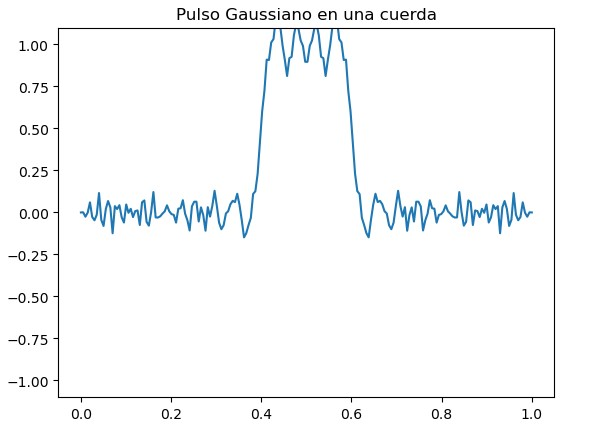
\includegraphics[width=0.7 \textwidth]{pul7.jpg}
    \caption{Modificación del pulso gaussiano en onda cuadrada.}
\end{figure}

\vspace{\baselineskip}

\begin{justify}
    \textbf{Comentarios del resultado:}
\end{justify}

\begin{itemize}
    \item La onda cuadrada muestra dispersión porque sus diferentes componentes de frecuencia viajan a velocidades ligeramente diferentes, además que se 
    se descompone rápidamente en una serie de ondas más complejas debido a que contiene más frecuencias (componentes de Fourier).
\end{itemize}

\section{Ejercicio 4: Ruptura de la velocidad del sonido.}

\begin{justify}
El ejercicio 4 de esta simulación consiste en ejecutar el código de una simulación del sonido que emite un jet supersónico, el cual viaja a una velocidad constante de \(1.5v_{s}\), donde \(v_{s}\) es la velocidad del sonido (Mach 1.5).
\end{justify}

\begin{enumerate}
    \item  Modifica el código para que el jet viaje a \(0.5v_{s}\), \(0.75v_{s}\), \(1.0v_{s}\) y \(2.0v_{s}\). Adjunta las imágenes resultantes y comenta cada uno de los resultados. Concretamente: ¿Qué pasa cuando la velocidad del jet es la velocidad del sonido? ¿Qué pasa si la excedemos?
    
    \item Aprovecha esta simulación para hacer una explicación del efecto Doppler. ¿Es válido el efecto Doppler cuando el objeto viaja a velocidades mayores a la velocidad del sonido? Argumenta tu respuesta con las fórmulas pertinentes.
    
    \item  Finalmente, realiza una última simulación donde la posición inicial es el origen de coordenadas y el jet está quieto, aunque emitiendo sonido. ¿Se recupera el resultado que esperabas?
\end{enumerate}

\subsection{Velocidad Jet.}

\begin{justify}
    \textbf{Gráfica  del jet cuando} \texttt{v\_s = 0.5}
\end{justify}

\begin{figure}[H]
    \centering
    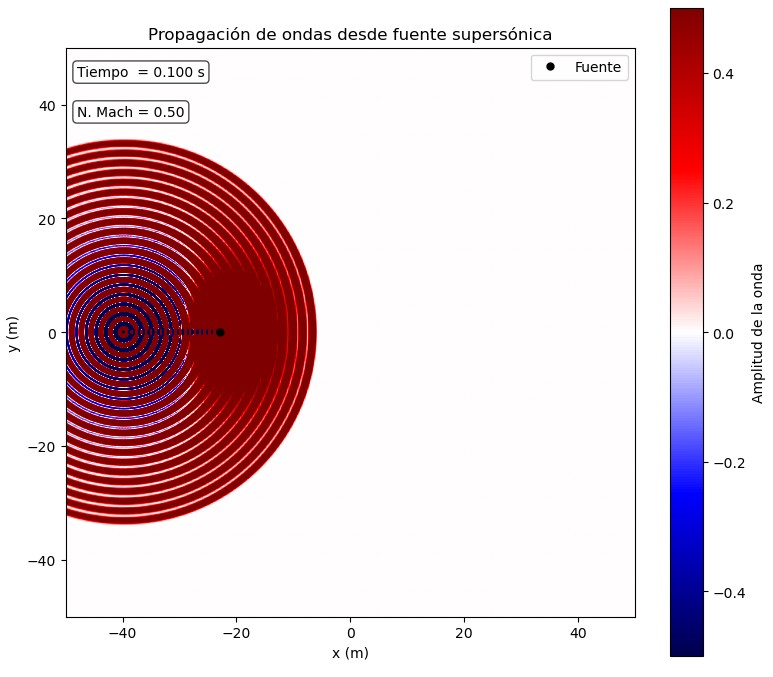
\includegraphics[width=0.8 \textwidth]{vel1.jpg}
\end{figure}

\begin{justify}
    Cuando \texttt{v\_s = 0.5} el jet se mueve \textbf{más lento que el sonido} (subsónico). La amplitud es mayor frente a la fuente (\textbf{efecto Doppler}) y menor detrás.
\end{justify}

\newpage

\begin{justify}
    \textbf{Gráfica  del jet cuando} \texttt{v\_s = 0.75}
\end{justify}

\begin{figure}[H]
    \centering
    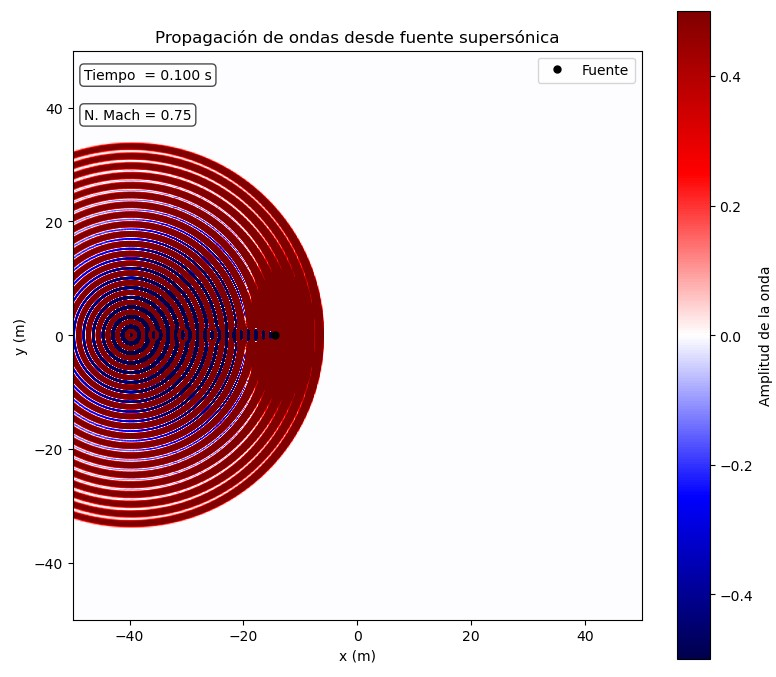
\includegraphics[width=0.9 \textwidth]{vel2.jpg}
\end{figure}

\vspace{\baselineskip}

\begin{justify}
    Cuando \texttt{v\_s = 0.75} se mueve  \textbf{más lento que el sonido} (subsónico), se comporta similar al punto pasado.
\end{justify}

\newpage

\begin{justify}
    \textbf{Gráfica  del jet cuando} \texttt{v\_s = 1.0}
\end{justify}


\begin{figure}[H]
    \centering
    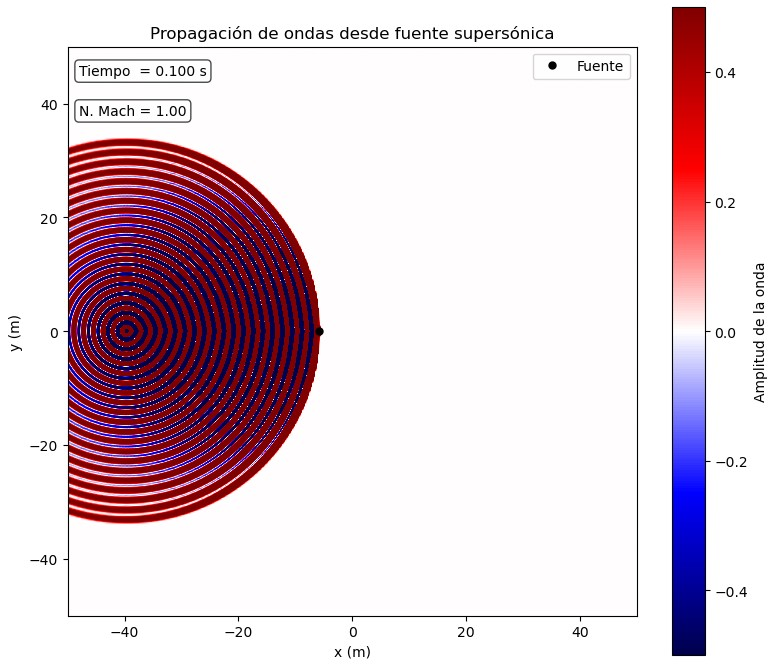
\includegraphics[width=0.9 \textwidth]{vel3.jpg}
\end{figure}


\vspace{\baselineskip}

\begin{justify}
    Cuando \texttt{v\_s = 1.0} se mueve  \textbf{a la misma velocidad que el sonido} (sónico). Las ondas emitidas se acumulan en el frente del jet, 
    creando  una interferencia constructiva en \(x = 0\).
\end{justify}

\newpage

\begin{justify}
    \textbf{Gráfica  del jet cuando} \texttt{v\_s = 2.0}
\end{justify}

\begin{figure}[H]
    \centering
    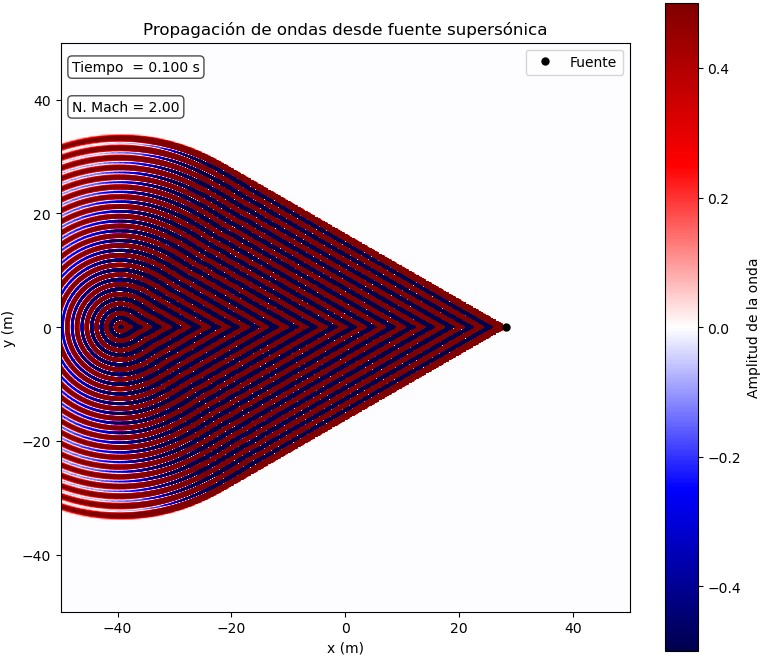
\includegraphics[width=0.9 \textwidth]{vel4.jpg}
\end{figure}

\vspace{\baselineskip}

\begin{justify}
    Cuando \texttt{v\_s = 2.0} se mueve  \textbf{más rapido que el sonido} (supersónico). LSe forma un cono de Mach (frente de choque).
\end{justify}

\vspace{\baselineskip}

\subsection{Interpretación efecto Doppler.}

\vspace{\baselineskip}

\begin{justify}
    Si el jet es más rápido que el sonido \texttt{v\_s > C}, la frecuencia percibida puede ser negativa o indefinida amtes de que la fuente pase al observador, además, el observador no escucharía nada hasta que el jet haya pasado su posición, en ese instante cuando el jet pasa, 
    se percibe un \textbf{boom sónico} que es una onda de choque, no una onda de sonido continua.
\end{justify}


\vspace{\baselineskip}


\subsection{Posición inicial en el origen de las coordenadas.}

\vspace{\baselineskip}

\begin{justify}
    Modificamos la velocidad \texttt{v\_s = 0} y el origen de coordenadas \texttt{x0 = 0}.
\end{justify}

\vspace{\baselineskip}

\begin{figure}[H]
    \centering
    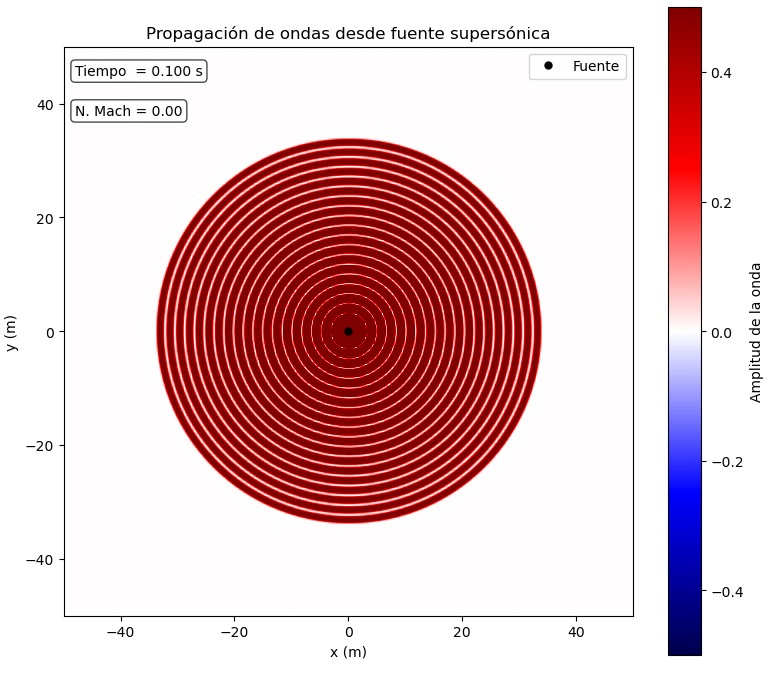
\includegraphics[width=0.9 \textwidth]{cod.1.jpg}
\end{figure}

\begin{justify}
    En este caso, las ondas deben propagrase de forma concéntrica, círculos simétricos alrededor del origen.
\end{justify}

\begin{justify}
    Si es lo que esperamos en la animación de este caso, dado que refleja como las ondas se expanden uniformemente, sin compresión o rarefacción en la dirección de movimiento.
\end{justify}


\section{Califiación/Observaciones.}

\vspace{\baselineskip}

\begin{figure}[H]
    \centering
    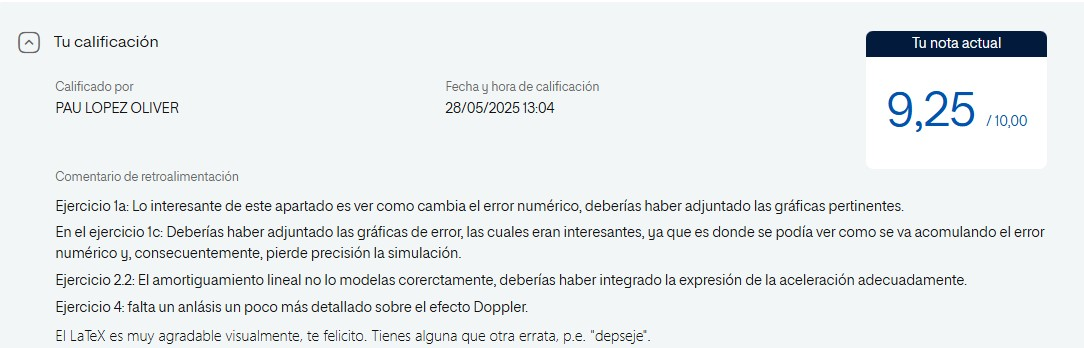
\includegraphics[width=1.1 \textwidth]{calificacion.jpg}
\end{figure}



\end{document}